\documentclass{article}
\usepackage[backend=biber,citestyle=ieee]{biblatex}
\usepackage[english]{babel}
%\usepackage[swedish]{babel}
\usepackage{graphicx}
\usepackage{csquotes}
\usepackage{float}
\usepackage{subcaption}
\usepackage{url}
\usepackage{float}
\usepackage{siunitx}
\usepackage{datetime}
\usepackage[title]{appendix}
\usepackage[font={small},margin={1cm}]{caption}
\usepackage{titlesec}
\usepackage{enumitem}
\usepackage{amsmath}
\usepackage{fancyhdr}   %page header
\usepackage[margin=1in]{geometry}
\setcounter{secnumdepth}{0}
\pagestyle{fancy}
\fancyhf{}

\cfoot{Page \thepage}

\usepackage[parfill]{parskip} %Line skip between paragraphs instead of indent

\usepackage{xcolor}
\usepackage{listings}   %code section 
\usepackage[hidelinks]{hyperref}



\newcommand{\getauthor}{Eric Johansson (erjo2002@student.miun.se)\\Can Kupeli (caku2002@student.miun.se) \\Samuel Greenberg (sagr1908@student.miun.se)} %Author
\newcommand{\gettitle}{Laboration 3 \\Markov Chains and Queue Theory} %Title
\newcommand{\getcourse}{(MA069G, Mathematical Modelling 6hp)} %Course
\newcommand{\getsupervisor}{Cornelia Schiebold\\Magnus Eriksson\\Suprokash Hazra}


\begin{document}
\begin{titlepage}
	\begin{center}
		\vspace*{1cm}

		
\includegraphics[width=0.8\textwidth]{imgs/msu.png}\\[0.5cm]
		\Large
		Institution of Information Systems and -Technology (IST)\\[1cm]
		\Huge
		\rule{\textwidth}{1px}
		\textbf{\gettitle}
		\rule[0.5cm]{\textwidth}{1px}

		\large
		\getcourse{}
		\vspace{1cm}

		\Large
		\textbf{\getauthor}\\

		\vfill


		\vspace{0.8cm}

		\small
		\today \\
		\Large
		\textbf{Supervisor:}\\
		\getsupervisor{}

	\end{center}
\end{titlepage}
\tableofcontents
\newpage
\lhead{Laboration 3}
\rhead{Eric, Can, Samuel}





\section{Question 1}
\subsection{(a)}
\begin{figure}[H]
        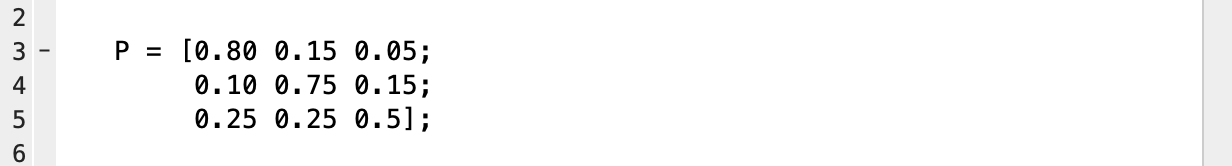
\includegraphics[width=\linewidth]{./imgs/1a.png}
        \caption{Transfer matrix for a current market simulation}
\end{figure}
The code shows the transfer matrix as an array where each collumn and row represent the transfer probability from each respective case.

\subsection{(b)}
\begin{figure}[H]
        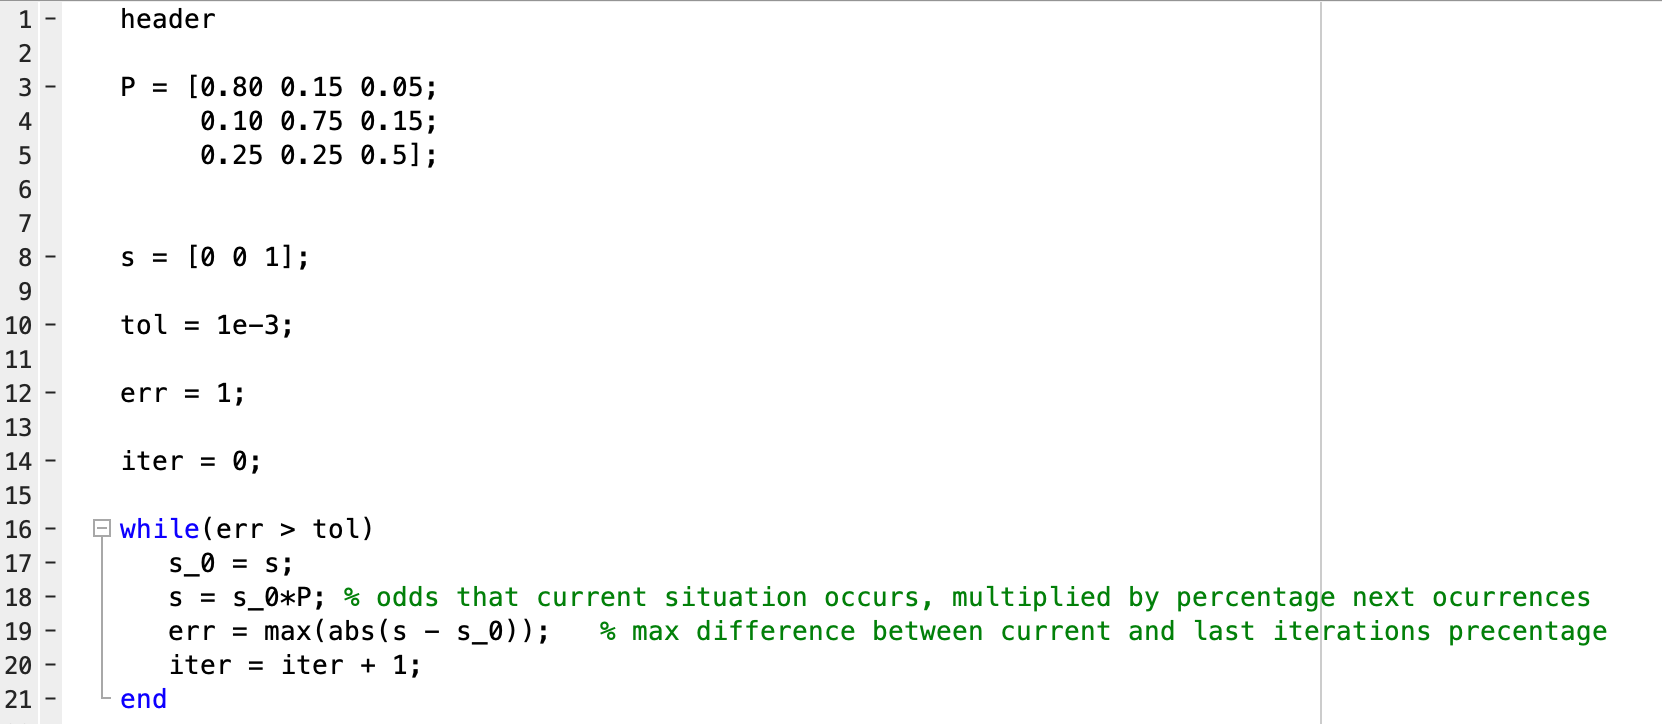
\includegraphics[width=\linewidth]{./imgs/1b.png}
        \caption{Simulation of a current market situation}
\end{figure}
The simulation is initiated with a recession, the error is calculated using the infinity norm (L$\infty$-norm), which is the max difference between the current and previous iteration's precentages.

\subsection{(c)}
\begin{figure}[H]
    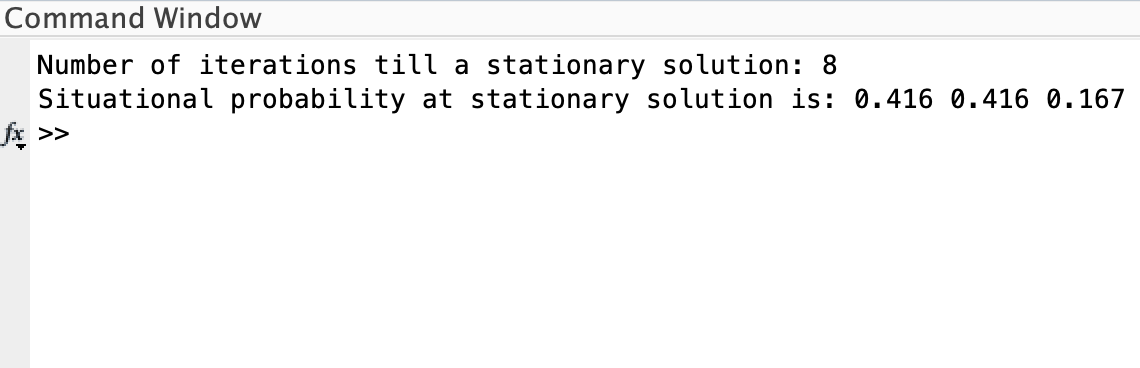
\includegraphics[width=\linewidth]{./imgs/1c.png}
    \caption{Number of iterations till and situational probability at a stationary solution}
\end{figure}

\subsection{(d)}
Given an adequate number of iterations, the probabilities will always converge to the same stationary value regardless of initial situation.

\subsection{(e)}
Recession leads to a stationary solution quicker than Bull and Bear.






\section{Question 2}
\begin{figure}[H]
    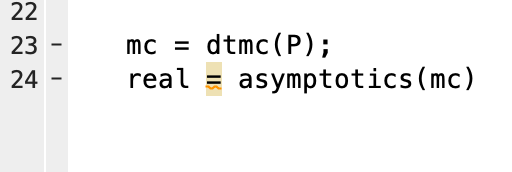
\includegraphics[width=\linewidth]{./imgs/2code.png}
    \caption{The functions used to calculate the exact probability}
\end{figure}
\begin{figure}[H]
    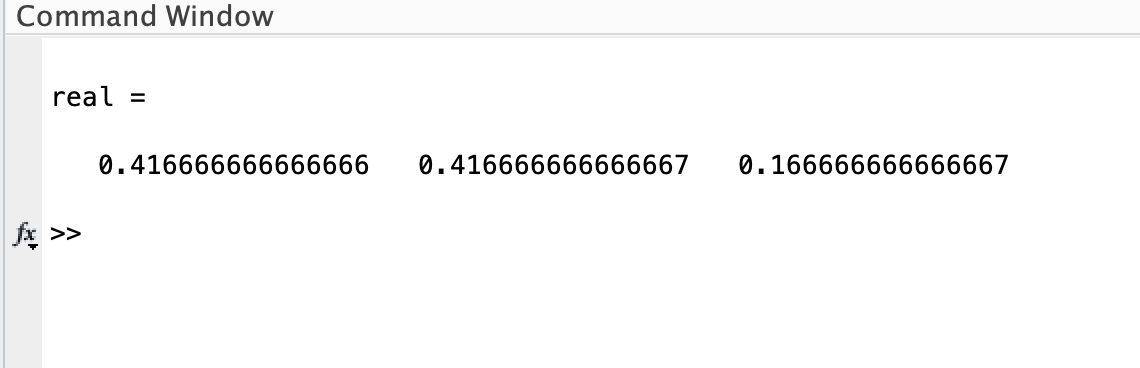
\includegraphics[width=\linewidth]{./imgs/2.png}
    \caption{The exact probabilities at the stationary solution, calculated using MatLabs built-in functions}
\end{figure}
The probability values from question 1 where verified by calculating the true value through both matlabs built-in functions and calculated for hand to be $\frac{5}{12} \frac{5}{12} \frac{1}{6}$.






\section{Question 3}
\begin{figure}[H]
    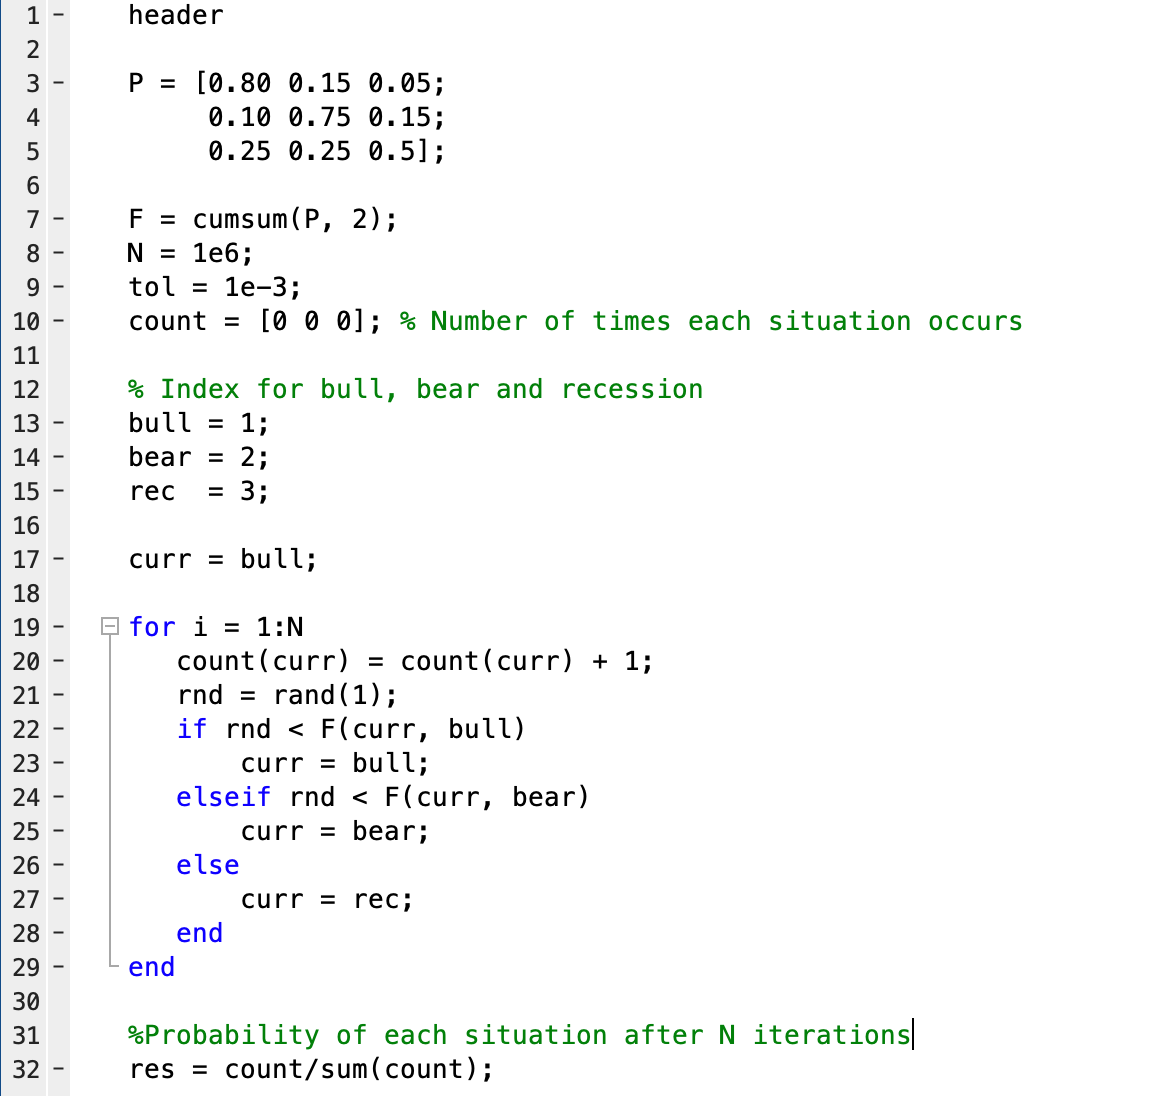
\includegraphics[width=\linewidth]{./imgs/3.png}
    \caption{Monte Carlo simulation of the Markov chain}
\end{figure}
\begin{figure}[H]
    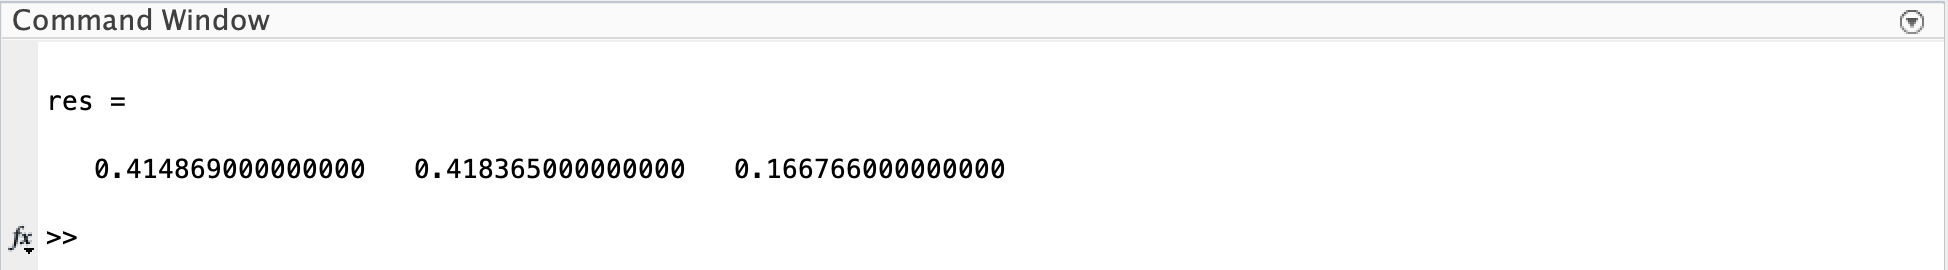
\includegraphics[width=\linewidth]{./imgs/3ans.png}
    \caption{The exact probabilities at the stationary solution, calculated using a Monte Carlo simulation}
    \label{fig:3ans}
\end{figure}
The simulation took 1 million iterations to get the results shown in Figure \ref{fig:3ans}. Considering that the method used in question one only required 8 iterations and resulted in a more accurate answer we can deduce that the Monte Carlo simulation was significantly slower and less accurate.





\section{Question 4}
\subsection{(a)}
\subsection{(b)}
\begin{figure}[H]
    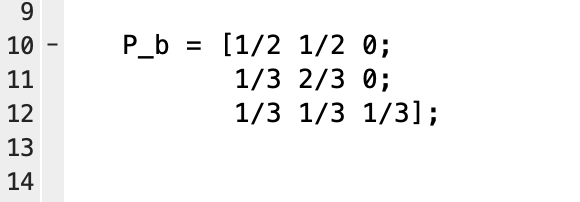
\includegraphics[width=\linewidth]{./imgs/4b.png}
    \caption{Reducible stochastic process}
\end{figure}
\subsection{(c)}
A none memorylessness process is where the steps are determined by the previous step or steps taken. An example of this would be that you cannot return to the previous situation, a recession cannot lead to a bear if the recession was preceded by a bear.
\subsection{(d)}
We believe B can work





\section{Question 5}
\subsection{(a)}
The M/M/2/4 is a Kendall notation, the first two variables represent the arrival and departure. The M's stands for Markov process, a poisson arrival (negative exponetial service). The third variable represents the number of servers, in this case 2. The fourth and final variable represents the buffer, the maximum number of customers allowed in the system, in this case 4.

\subsection{(b)}
\begin{figure}[H]
    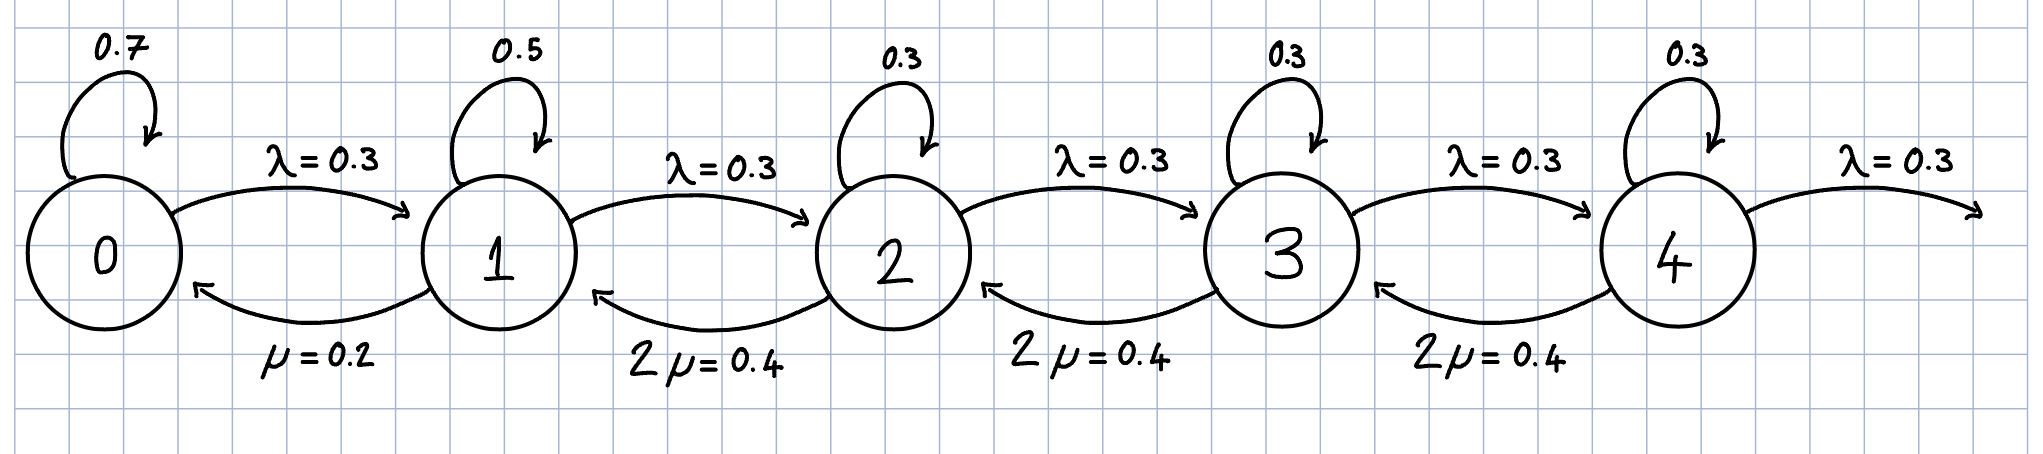
\includegraphics[width=\linewidth]{./imgs/5b.JPG}
    \caption{Markov Chains state diagram with transition probabilities}
\end{figure}

\subsection{(c)}
\begin{figure}[H]
    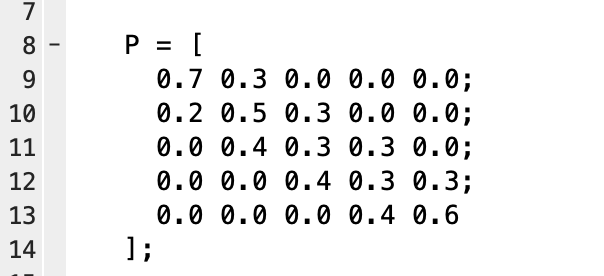
\includegraphics[width=\linewidth]{./imgs/5c.png}
    \caption{Transfer matrix}
\end{figure}

\subsection{(d)}
\begin{figure}[H]
    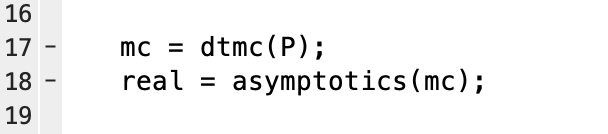
\includegraphics[width=\linewidth]{./imgs/5dcode.png}
    \caption{The functions used to calculate the exact probability}
\end{figure}
\begin{figure}[H]
    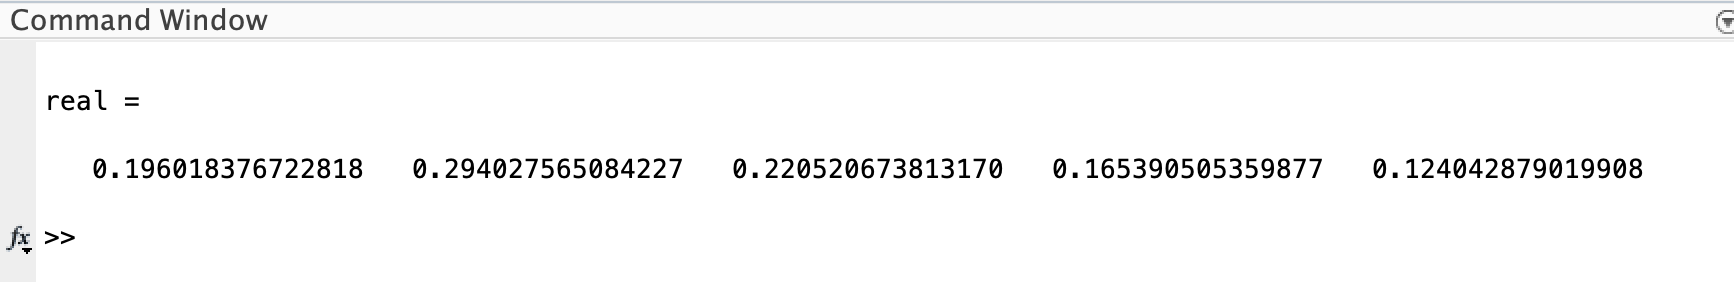
\includegraphics[width=\linewidth]{./imgs/5dans.png}
    \caption{The exact probabilities at the stationary solution}
\end{figure}

\subsection{(e)}
\begin{figure}[H]
    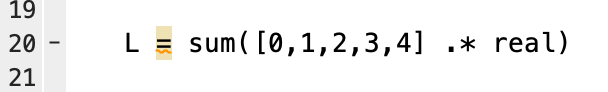
\includegraphics[width=\linewidth]{./imgs/5ecode.png}
    \caption{Function used to calculate average number of customers in the system}
\end{figure}
\begin{figure}[H]
    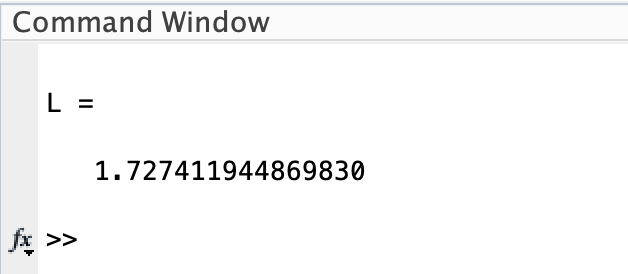
\includegraphics[width=\linewidth]{./imgs/5eans.png}
    \caption{Average number of customers in the system}
\end{figure}

\subsection{(f)}
\begin{figure}[H]
    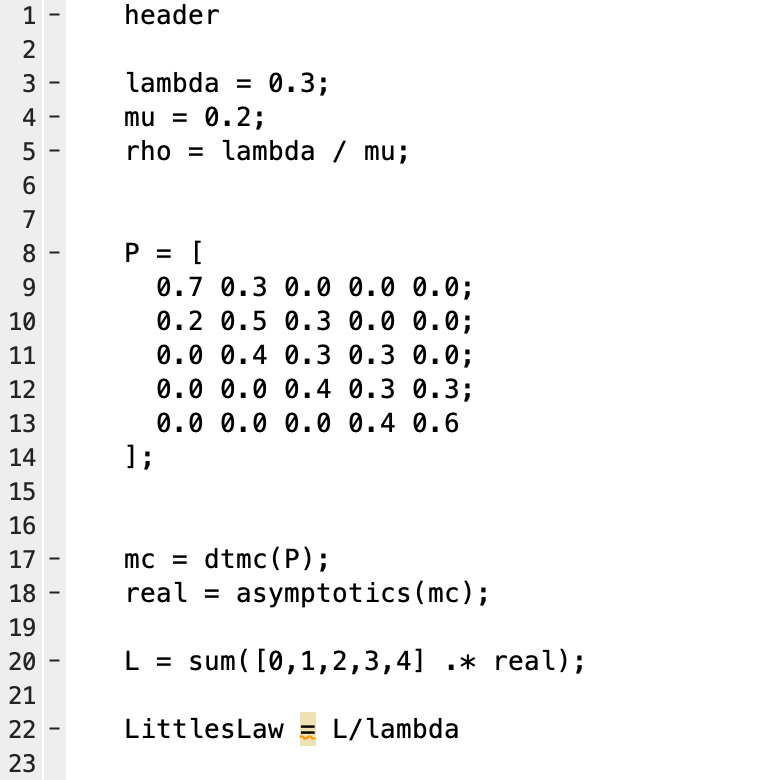
\includegraphics[width=\linewidth]{./imgs/5fcode.png}
    \caption{Method used to calculate the average time a customer spends in the system}
\end{figure}
\begin{figure}[H]
    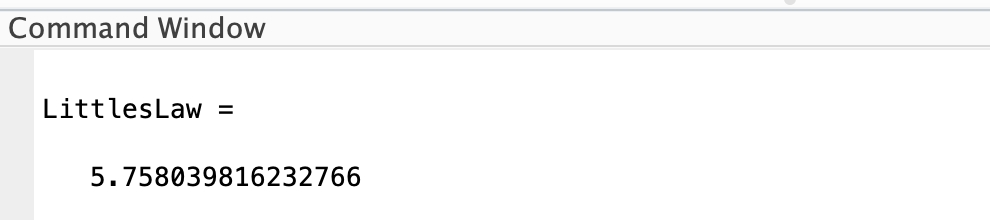
\includegraphics[width=\linewidth]{./imgs/5fans.png}
    \caption{Average time a customer spends in the system}
\end{figure}
Using Little's Law the average time a customer spends within the system is calculated to 5.76 minutes. 
This was done by dividing the average number of customers in the system by the customer arrival rate.




\end{document}
